%-----------------------------------------------------------------------------
% PACKAGES AND OTHER DOCUMENT CONFIGURATIONS
%-----------------------------------------------------------------------------

\documentclass[11pt,addpoints,answers]{exam}
\usepackage[margin=1in]{geometry}
\usepackage{amsmath, amsfonts}
\usepackage{enumerate}
\usepackage{graphicx}
\usepackage{titling}
\usepackage{url}
\usepackage{xfrac}
\usepackage{natbib}
\usepackage{amssymb}
\usepackage{amsthm}
\usepackage{paralist}
\usepackage{epstopdf}
\usepackage{tabularx}
\usepackage{longtable}
\usepackage{multirow}
\usepackage{multicol}
\usepackage[colorlinks=true,urlcolor=blue]{hyperref}
\usepackage{algorithm}
\usepackage{algorithmicx}
\usepackage[noend]{algpseudocode}
\usepackage{float}
\usepackage{enumerate}
\usepackage{array}
\usepackage{environ}
\usepackage{times}
\usepackage{textcomp}
\usepackage{caption}
\usepackage{parskip} % For NIPS style paragraphs.
\usepackage[compact]{titlesec} % Less whitespace around titles
\usepackage{titling}
\setlength{\droptitle}{-2cm}
\usepackage[inline]{enumitem} % For inline enumerate* and itemize*
\usepackage{datetime}
\usepackage{comment}
% \usepackage{minted}
\usepackage{lastpage}
\usepackage{color}
\usepackage{xcolor}
\usepackage[final]{listings}
\usepackage{tikz}
\usetikzlibrary{shapes,decorations}
\usepackage{framed}
\usepackage{booktabs}
\usepackage{cprotect}
\usepackage{verbatimbox}
\usepackage{multicol}
\usepackage{hyperref}
\usepackage{subcaption}
\usepackage{mathtools} % For drcases
\usepackage{cancel}
\usepackage[many]{tcolorbox}
\usepackage{soul}
\usepackage{tikz}
\usepackage{wasysym}
\usepackage{mdsymbol}
\usepackage{transparent}

\usetikzlibrary{shapes.geometric}
\usetikzlibrary{positioning, arrows, automata}

\newtcolorbox[]{your_solution}[1][]{%
    % breakable,
    enhanced,
    nobeforeafter,
    colback=white,
    title=Your Answer,
    sidebyside align=top,
    box align=top,
    #1
}

%%%%%%%%%%%%%%%%%%%%%%%%%%%%%%%%%%%%%%%%%%%
% Better numbering                        %
%%%%%%%%%%%%%%%%%%%%%%%%%%%%%%%%%%%%%%%%%%%

% \numberwithin{equation}{section} % Number equations within sections (i.e. 1.1, 1.2, 2.1, 2.2 instead of 1, 2, 3, 4)
% \numberwithin{figure}{section} % Number figures within sections (i.e. 1.1, 1.2, 2.1, 2.2 instead of 1, 2, 3, 4)
% \numberwithin{table}{section} % Number tables within sections (i.e. 1.1, 1.2, 2.1, 2.2 instead of 1, 2, 3, 4)

%%%%%%%%%%%%%%%%%%%%%%%%%%%%%%%%%%%%%%%%%%
% Custom commands                        %
%%%%%%%%%%%%%%%%%%%%%%%%%%%%%%%%%%%%%%%%%%
\newcommand{\blackcircle}{\tikz\draw[black,fill=black] (0,0) circle (1ex);}
\renewcommand{\circle}{\tikz\draw[black] (0,0) circle (1ex);}
\newcommand{\vc}[1]{\boldsymbol{#1}}
\newcommand{\adj}[1]{\frac{\partial \ell}{\partial #1}}
\newcommand{\chain}[2]{\adj{#2} = \adj{#1}\frac{\partial #1}{\partial #2}}
\newcommand{\ntset}{test}

% mathcal
\newcommand{\Ac}{\mathcal{A}}
\newcommand{\Bc}{\mathcal{B}}
\newcommand{\Cc}{\mathcal{C}}
\newcommand{\Dc}{\mathcal{D}}
\newcommand{\Ec}{\mathcal{E}}
\newcommand{\Fc}{\mathcal{F}}
\newcommand{\Gc}{\mathcal{G}}
\newcommand{\Hc}{\mathcal{H}}
\newcommand{\Ic}{\mathcal{I}}
\newcommand{\Jc}{\mathcal{J}}
\newcommand{\Kc}{\mathcal{K}}
\newcommand{\Lc}{\mathcal{L}}
\newcommand{\Mc}{\mathcal{M}}
\newcommand{\Nc}{\mathcal{N}}
\newcommand{\Oc}{\mathcal{O}}
\newcommand{\Pc}{\mathcal{P}}
\newcommand{\Qc}{\mathcal{Q}}
\newcommand{\Rc}{\mathcal{R}}
\newcommand{\Sc}{\mathcal{S}}
\newcommand{\Tc}{\mathcal{T}}
\newcommand{\Uc}{\mathcal{U}}
\newcommand{\Vc}{\mathcal{V}}
\newcommand{\Wc}{\mathcal{W}}
\newcommand{\Xc}{\mathcal{X}}
\newcommand{\Yc}{\mathcal{Y}}
\newcommand{\Zc}{\mathcal{Z}}

% mathbb
\newcommand{\Ab}{\mathbb{A}}
\newcommand{\Bb}{\mathbb{B}}
\newcommand{\Cb}{\mathbb{C}}
\newcommand{\Db}{\mathbb{D}}
\newcommand{\Eb}{\mathbb{E}}
\newcommand{\Fb}{\mathbb{F}}
\newcommand{\Gb}{\mathbb{G}}
\newcommand{\Hb}{\mathbb{H}}
\newcommand{\Ib}{\mathbb{I}}
\newcommand{\Jb}{\mathbb{J}}
\newcommand{\Kb}{\mathbb{K}}
\newcommand{\Lb}{\mathbb{L}}
\newcommand{\Mb}{\mathbb{M}}
\newcommand{\Nb}{\mathbb{N}}
\newcommand{\Ob}{\mathbb{O}}
\newcommand{\Pb}{\mathbb{P}}
\newcommand{\Qb}{\mathbb{Q}}
\newcommand{\Rb}{\mathbb{R}}
\newcommand{\Sb}{\mathbb{S}}
\newcommand{\Tb}{\mathbb{T}}
\newcommand{\Ub}{\mathbb{U}}
\newcommand{\Vb}{\mathbb{V}}
\newcommand{\Wb}{\mathbb{W}}
\newcommand{\Xb}{\mathbb{X}}
\newcommand{\Yb}{\mathbb{Y}}
\newcommand{\Zb}{\mathbb{Z}}

% mathbf lowercase
\newcommand{\av}{\mathbf{a}}
\newcommand{\bv}{\mathbf{b}}
\newcommand{\cv}{\mathbf{c}}
\newcommand{\dv}{\mathbf{d}}
\newcommand{\ev}{\mathbf{e}}
\newcommand{\fv}{\mathbf{f}}
\newcommand{\gv}{\mathbf{g}}
\newcommand{\hv}{\mathbf{h}}
\newcommand{\iv}{\mathbf{i}}
\newcommand{\jv}{\mathbf{j}}
\newcommand{\kv}{\mathbf{k}}
\newcommand{\lv}{\mathbf{l}}
\newcommand{\mv}{\mathbf{m}}
\newcommand{\nv}{\mathbf{n}}
\newcommand{\ov}{\mathbf{o}}
\newcommand{\pv}{\mathbf{p}}
\newcommand{\qv}{\mathbf{q}}
\newcommand{\rv}{\mathbf{r}}
\newcommand{\sv}{\mathbf{s}}
\newcommand{\tv}{\mathbf{t}}
\newcommand{\uv}{\mathbf{u}}
\newcommand{\vv}{\mathbf{v}}
\newcommand{\wv}{\mathbf{w}}
\newcommand{\xv}{\mathbf{x}}
\newcommand{\yv}{\mathbf{y}}
\newcommand{\zv}{\mathbf{z}}

% mathbf uppercase
\newcommand{\Av}{\mathbf{A}}
\newcommand{\Bv}{\mathbf{B}}
\newcommand{\Cv}{\mathbf{C}}
\newcommand{\Dv}{\mathbf{D}}
\newcommand{\Ev}{\mathbf{E}}
\newcommand{\Fv}{\mathbf{F}}
\newcommand{\Gv}{\mathbf{G}}
\newcommand{\Hv}{\mathbf{H}}
\newcommand{\Iv}{\mathbf{I}}
\newcommand{\Jv}{\mathbf{J}}
\newcommand{\Kv}{\mathbf{K}}
\newcommand{\Lv}{\mathbf{L}}
\newcommand{\Mv}{\mathbf{M}}
\newcommand{\Nv}{\mathbf{N}}
\newcommand{\Ov}{\mathbf{O}}
\newcommand{\Pv}{\mathbf{P}}
\newcommand{\Qv}{\mathbf{Q}}
\newcommand{\Rv}{\mathbf{R}}
\newcommand{\Sv}{\mathbf{S}}
\newcommand{\Tv}{\mathbf{T}}
\newcommand{\Uv}{\mathbf{U}}
\newcommand{\Vv}{\mathbf{V}}
\newcommand{\Wv}{\mathbf{W}}
\newcommand{\Xv}{\mathbf{X}}
\newcommand{\Yv}{\mathbf{Y}}
\newcommand{\Zv}{\mathbf{Z}}

% bold greek lowercase
\newcommand{\alphav     }{\boldsymbol \alpha     }
\newcommand{\betav      }{\boldsymbol \beta      }
\newcommand{\gammav     }{\boldsymbol \gamma     }
\newcommand{\deltav     }{\boldsymbol \delta     }
\newcommand{\epsilonv   }{\boldsymbol \epsilon   }
\newcommand{\varepsilonv}{\boldsymbol \varepsilon}
\newcommand{\zetav      }{\boldsymbol \zeta      }
\newcommand{\etav       }{\boldsymbol \eta       }
\newcommand{\thetav     }{\boldsymbol \theta     }
\newcommand{\varthetav  }{\boldsymbol \vartheta  }
\newcommand{\iotav      }{\boldsymbol \iota      }
\newcommand{\kappav     }{\boldsymbol \kappa     }
\newcommand{\varkappav  }{\boldsymbol \varkappa  }
\newcommand{\lambdav    }{\boldsymbol \lambda    }
\newcommand{\muv        }{\boldsymbol \mu        }
\newcommand{\nuv        }{\boldsymbol \nu        }
\newcommand{\xiv        }{\boldsymbol \xi        }
\newcommand{\omicronv   }{\boldsymbol \omicron   }
\newcommand{\piv        }{\boldsymbol \pi        }
\newcommand{\varpiv     }{\boldsymbol \varpi     }
\newcommand{\rhov       }{\boldsymbol \rho       }
\newcommand{\varrhov    }{\boldsymbol \varrho    }
\newcommand{\sigmav     }{\boldsymbol \sigma     }
\newcommand{\varsigmav  }{\boldsymbol \varsigma  }
\newcommand{\tauv       }{\boldsymbol \tau       }
\newcommand{\upsilonv   }{\boldsymbol \upsilon   }
\newcommand{\phiv       }{\boldsymbol \phi       }
\newcommand{\varphiv    }{\boldsymbol \varphi    }
\newcommand{\chiv       }{\boldsymbol \chi       }
\newcommand{\psiv       }{\boldsymbol \psi       }
\newcommand{\omegav     }{\boldsymbol \omega     }

% bold greek uppercase
\newcommand{\Gammav     }{\boldsymbol \Gamma     }
\newcommand{\Deltav     }{\boldsymbol \Delta     }
\newcommand{\Thetav     }{\boldsymbol \Theta     }
\newcommand{\Lambdav    }{\boldsymbol \Lambda    }
\newcommand{\Xiv        }{\boldsymbol \Xi        }
\newcommand{\Piv        }{\boldsymbol \Pi        }
\newcommand{\Sigmav     }{\boldsymbol \Sigma     }
\newcommand{\Upsilonv   }{\boldsymbol \Upsilon   }
\newcommand{\Phiv       }{\boldsymbol \Phi       }
\newcommand{\Psiv       }{\boldsymbol \Psi       }
\newcommand{\Omegav     }{\boldsymbol \Omega     }

%%%%%%%%%%%%%%%%%%%%%%%%%%%%%%%%%%%%%%%%%%%
% Code highlighting with listings         %
%%%%%%%%%%%%%%%%%%%%%%%%%%%%%%%%%%%%%%%%%%%

\definecolor{bluekeywords}{rgb}{0.13,0.13,1}
\definecolor{greencomments}{rgb}{0,0.5,0}
\definecolor{redstrings}{rgb}{0.9,0,0}
\definecolor{light-gray}{gray}{0.95}

\newcommand{\MYhref}[3][blue]{\href{#2}{\color{#1}{#3}}}%

\definecolor{dkgreen}{rgb}{0,0.6,0}
\definecolor{gray}{rgb}{0.5,0.5,0.5}
\definecolor{mauve}{rgb}{0.58,0,0.82}

\lstdefinelanguage{Shell}{
  keywords={tar, cd, make},
  %keywordstyle=\color{bluekeywords}\bfseries,
  alsoletter={+},
  ndkeywords={python3, python, py, javac, java, gcc, c, g++, cpp, .txt, octave, m, .tar},
  %ndkeywordstyle=\color{bluekeywords}\bfseries,
  identifierstyle=\color{black},
  sensitive=false,
  comment=[l]{//},
  morecomment=[s]{/*}{*/},
  commentstyle=\color{purple}\ttfamily,
  %stringstyle=\color{red}\ttfamily,
  morestring=[b]',
  morestring=[b]",
  backgroundcolor = \color{light-gray}
}

\lstset{columns=fixed, basicstyle=\ttfamily,
    backgroundcolor=\color{light-gray},xleftmargin=0.5cm,frame=tlbr,framesep=4pt,framerule=0pt}

\newcommand{\emptysquare}{{\LARGE $\square$}\ \ }
\newcommand{\filledsquare}{{\LARGE $\boxtimes$}\ \ }
\def \ifempty#1{\def\temp{#1} \ifx\temp\empty }


% \newcommand{\squaresolutionspace}[2][\emptysquare]{\newline #1}{#2}
\def \squaresolutionspace#1{ \ifempty{#1} \emptysquare \else #1\hspace{0.75pt}\fi}


\newcommand{\emptycircle}{{\LARGE $\fullmoon$}\ \ }
\newcommand{\filledcircle}{{\LARGE $\newmoon$}\ \ }
\def \circlesolutionspace#1{ \ifempty{#1} \emptycircle \else #1\hspace{0.75pt}\fi}
%%%%%%%%%%%%%%%%%%%%%%%%%%%%%%%%%%%%%%%%%%%
% Custom box for highlights               %
%%%%%%%%%%%%%%%%%%%%%%%%%%%%%%%%%%%%%%%%%%%

% Define box and box title style
\tikzstyle{mybox} = [fill=blue!10, very thick,
    rectangle, rounded corners, inner sep=1em, inner ysep=1em]

% \newcommand{\notebox}[1]{
% \begin{tikzpicture}
% \node [mybox] (box){%
%     \begin{minipage}{\textwidth}
%     #1
%     \end{minipage}
% };
% \end{tikzpicture}%
% }

\NewEnviron{notebox}{
\begin{tikzpicture}
\node [mybox] (box){
    \begin{minipage}{0.95\textwidth}
        \BODY
    \end{minipage}
};
\end{tikzpicture}
}

%%%%%%%%%%%%%%%%%%%%%%%%%%%%%%%%%%%%%%%%%%%
% Commands showing / hiding solutions     %
%%%%%%%%%%%%%%%%%%%%%%%%%%%%%%%%%%%%%%%%%%%
\newcommand{\solutionspace}[4]{\fbox{\begin{minipage}[t][#1][t]{#2} \textbf{#3} \solution{}{#4} \end{minipage}}}
%% To HIDE SOLUTIONS (to post at the website for students), set this value to 0: \def\issoln{0}
\def\issoln{1}
%\def\issoln{1}
% Some commands to allow solutions to be embedded in the assignment file.
\ifcsname issoln\endcsname \else \def\issoln{1} \fi
% Default to an empty solutions environ.
\NewEnviron{soln}{}{}
\if\issoln 1
% Otherwise, include solutions as below.
\RenewEnviron{soln}{
    \leavevmode\color{red}\ignorespaces
    % \textbf{Solution} \BODY
    \BODY
}{}
\fi

%% To HIDE TAGS set this value to 0:
\def\showtags{1}
%%%%%%%%%%%%%%%%
\ifcsname showtags\endcsname \else \def\showtags{1} \fi
% Default to an empty tags environ.
\NewEnviron{tags}{}{}
\if\showtags 1
% Otherwise, include solutions as below.
\RenewEnviron{tags}{
    \fbox{
    \leavevmode\color{blue}\ignorespaces
    \textbf{TAGS:} \texttt{\url{\BODY}}
    }
    \vspace{-.5em}
}{}
\fi

%%%%%%%%%%%%%%%%%%%%%%%%%%%%%%%%%%%%%%%%%%%
% Commands for customizing the assignment %
%%%%%%%%%%%%%%%%%%%%%%%%%%%%%%%%%%%%%%%%%%%

\newcommand{\courseNum}{10-301 / 10-601}
\newcommand{\courseName}{Introduction to Machine Learning}
\newcommand{\courseSem}{Fall 2021}
\newcommand{\courseUrl}{\url{http://mlcourse.org}}
\newcommand{\hwNum}{Homework 2}
\newcommand{\hwTopic}{Decision Trees}
\newcommand{\hwName}{\hwNum: \hwTopic}
\newcommand{\outDate}{Sept. 8, 2021}
\newcommand{\dueDate}{Sept. 20, 2021}
\newcommand{\taNames}{Catherine, Zachary, Ari, Siyuan, Anoushka}

%\pagestyle{fancyplain}
\lhead{\hwName}
\rhead{\courseNum}
\cfoot{\thepage{} of \numpages{}}

\title{\textsc{\hwNum}\\
\textsc{\hwTopic}
\thanks{Compiled on \today{} at \currenttime{}}\\
\vspace{1em}
} % Title


\author{\textsc{\large \courseNum{} \courseName{} (\courseSem)}\\
\courseUrl
\vspace{1em}\\
  OUT: \outDate \\
  DUE: \dueDate \\
  TAs: \taNames\\
}

\date{}

%%%%%%%%%%%%%%%%%%%%%%%%%%%%%%%%%%%%%%%%%%%%%%%%%
% Useful commands for typesetting the questions %
%%%%%%%%%%%%%%%%%%%%%%%%%%%%%%%%%%%%%%%%%%%%%%%%%

\newcommand \expect {\mathbb{E}}
\newcommand \mle [1]{{\hat #1}^{\rm MLE}}
\newcommand \map [1]{{\hat #1}^{\rm MAP}}
\newcommand \argmax {\operatorname*{argmax}}
\newcommand \argmin {\operatorname*{argmin}}
\newcommand \code [1]{{\tt #1}}
\newcommand \datacount [1]{\#\{#1\}}
\newcommand \ind [1]{\mathbb{I}\{#1\}}
% \renewcommand{\questionlabel}{(\alph{question})}

%%%%%%%%%%%%%%%%%%%%%%%%%%
% Document configuration %
%%%%%%%%%%%%%%%%%%%%%%%%%%

% Don't display a date in the title and remove the white space
\predate{}
\postdate{}
\date{}

% Don't display an author and remove the white space
%\preauthor{}
%\postauthor{}

%%%%%%%%%%%%%%%%%%
% Custom %
%%%%%%%%%%%%%%%%%% 

%%%%%%%%%%%%%%%%%%%%%%%%%%%%%%%%%%%%%%%%%%%
% Formatting for \CorrectChoice of "exam" %
%%%%%%%%%%%%%%%%%%%%%%%%%%%%%%%%%%%%%%%%%%%

\CorrectChoiceEmphasis{}
\checkedchar{\blackcircle}
\begin{document}

\maketitle

\begin{notebox}
\paragraph{Summary} It's time to build your first end-to-end learning system! In this assignment, you will build a Decision Tree classifier and apply it to several binary classification problems. This assignment consists of several parts: In Written component, you will work through some Information Theory basics in order to ``learn'' a Decision Tree on paper. Then in Programming component, you will implement Decision Tree learning, prediction, and evaluation. Using that implementation, you will answer the empirical questions found at the end of the Written component.
\end{notebox}
\section*{START HERE: Instructions}
\begin{itemize}

\item \textbf{Collaboration Policy}: Please read the collaboration policy here: \url{http://www.cs.cmu.edu/~mgormley/courses/10601/syllabus.html}

\item\textbf{Late Submission Policy:} See the late submission policy here: \url{http://www.cs.cmu.edu/~mgormley/courses/10601/syllabus.html}

\item\textbf{Submitting your work:} You will use Gradescope to submit
  answers to all questions and code. Please
  follow instructions at the end of this PDF to correctly submit all your code to Gradescope.

  \begin{itemize}
    
 % COMMENT IF NOT USING CANVAS
\begin{comment}
  \item \textbf{Canvas:} Canvas (\url{https://canvas.cmu.edu}) will be
    used for quiz-style problems (e.g. multiple choice, true / false,
    numerical answers). Grading is done automatically.
    %
    You may only \textbf{submit once} on canvas, so be sure of your
    answers before you submit. However, canvas allows you to work on
    your answers and then close out of the page and it will save your
    progress.  You will not be granted additional submissions, so
    please be confident of your solutions when you are submitting your
    assignment.
    %
    {\color{red} The above is true for future assignments, but this one
    allows {\bf unlimited submissions}.}
\end{comment}
    
  % COMMENT IF NOT USING GRADESCOPE
   \item \textbf{Written:} For written problems such as short answer, multiple choice, derivations, proofs, or plots, please use the provided template. Submissions can be handwritten onto the template, but should be labeled and clearly legible. If your writing is not legible, you will not be awarded marks. Alternatively, submissions can be written in LaTeX. 
   Each derivation/proof should be completed in the boxes provided. If you do not follow the template, your assignment may not be graded correctly by our AI assisted grader.

  %   COMMENT IF NOT USING GRADESCOPE AUTOGRADER
  \item \textbf{Programming:} You will submit your code for programming questions on the homework to Gradescope (\url{https://gradescope.com}). After uploading your code, our grading scripts will autograde your assignment by running your program on a virtual machine (VM). When you are developing, check that the version number of the programming language environment (e.g. Python 3.9.6, OpenJDK 11.0.11, g++ 7.5.0) and versions of permitted libraries (e.g.  \texttt{numpy} 1.21.2 and \texttt{scipy} 1.7.1) match those used on Gradescope. You have 10 Gradescope programming submissions. We recommend debugging your implementation on your local machine (or the Linux servers) and making sure your code is running correctly first before submitting you code to Gradescope.

  \end{itemize}
  
\item\textbf{Materials:} The data that you will need in order to complete this assignment is posted along with the writeup and template on Piazza.

\end{itemize}


\begin{notebox}
\paragraph{Linear Algebra Libraries} When implementing machine learning algorithms, it is often convenient to have a linear algebra library at your disposal. In this assignment, Java users may use EJML\footnote{\url{https://ejml.org}} or ND4J\footnote{\url{https://javadoc.io/doc/org.nd4j/nd4j-api/latest/index.html}} and C++ users may use Eigen\footnote{\url{http://eigen.tuxfamily.org/}}. Details below. 
%
(As usual, Python users have NumPy.)
%
\begin{description}
\item[EJML for Java] EJML is a pure Java linear algebra package with three interfaces. We strongly recommend using the SimpleMatrix interface. The autograder will use EJML version 0.41. When compiling and running your code, we will add the additional command line argument {\footnotesize{\lstinline{-cp "linalg_lib/ejml-v0.41-libs/*:linalg_lib/nd4j-v1.0.0-M1.1-libs/*:./"}}}
to ensure that all the EJML jars are on the classpath as well as your code. 

\item[ND4J for Java] ND4J is a library for multidimensional tensors with an interface akin to Python's NumPy. The autograder will use ND4J version 1.0.0-M1.1. When compiling and running your code, we will add the additional command line argument {\footnotesize{\lstinline{-cp "linalg_lib/ejml-v0.41-libs/*:linalg_lib/nd4j-v1.0.0-M1.1-libs/*:./"}}} to ensure that all the ND4J jars are on the classpath as well as your code. 

\item[Eigen for C++] Eigen is a header-only library, so there is no linking to worry about---just \lstinline{#include} whatever components you need. The autograder will use Eigen version 3.4.0. The command line arguments above demonstrate how we will call you code. When compiling your code we will include, the argument \lstinline{-I./linalg_lib} in order to include the \lstinline{linalg_lib/Eigen} subdirectory, which contains all the headers.

\end{description} 
We have included the correct versions of EJML/ND4J/Eigen in the \lstinline{linalg_lib.zip} posted on the Coursework page of the course website for your convenience. It contains the same \lstinline{linalg_lib/} directory that we will include in the current working directory when running your tests. Do {\bf not} include EJML, ND4J, or Eigen in your homework submission; the autograder will ensure that they are in place. 
\end{notebox}\clearpage

\section*{Instructions for Specific Problem Types}

For ``Select One" questions, please fill in the appropriate bubble completely:

\begin{quote}
\textbf{Select One:} Who taught this course?
     \begin{checkboxes}
     \CorrectChoice Matt Gormley / Henry Chai
     \choice Marie Curie
     \choice Noam Chomsky
    \end{checkboxes}
\end{quote}

If you need to change your answer, you may cross out the previous answer and bubble in the new answer:

\begin{quote}
\textbf{Select One:} Who taught this course?
\begin{list}{}
     \item\CIRCLE{} Matt Gormley / Henry Chai
     \item\Circle{} Marie Curie\\
     \xcancel{\CIRCLE}{} Noam Chomsky
\end{list}
\end{quote}


For ``Select all that apply" questions, please fill in all appropriate squares completely:

\begin{quote}
\textbf{Select all that apply:} Which are scientists?
{
    \checkboxchar{$\Box$} \checkedchar{$\blacksquare$}
    \begin{checkboxes}
     \choice Stephen Hawking 
     \CorrectChoice Albert Einstein
     \choice Isaac Newton
     \choice None of the above
    \end{checkboxes}
    }
\end{quote}

Again, if you need to change your answer, you may cross out the previous answer(s) and bubble in the new answer(s):

\begin{quote}
\textbf{Select all that apply:} Which are scientists?
    \begin{list}{}
    \item $\blacksquare$ Stephen Hawking 
    \item $\blacksquare$ Albert Einstein
    \item $\blacksquare$ Isaac Newton\\
    \xcancel{$\blacksquare$} I don't know
\end{list}
\end{quote}

For questions where you must fill in a blank, please make sure your final answer is fully included in the given space. You may cross out answers or parts of answers, but the final answer must still be within the given space.

\begin{quote}
\textbf{Fill in the blank:} What is the course number?

\begin{tcolorbox}[fit,height=1cm, width=4cm, blank, borderline={1pt}{-2pt},nobeforeafter]
    \begin{center}\huge10-601\end{center}
    \end{tcolorbox}\hspace{2cm}
    \begin{tcolorbox}[fit,height=1cm, width=4cm, blank, borderline={1pt}{-2pt},nobeforeafter]
    \begin{center}\huge10-\xcancel{7}601\end{center}
    \end{tcolorbox}
\end{quote}

\clearpage
\clearpage

\section{Written Questions (30 points)}
\subsection{Warm-Up}

First, let's think a little bit about decision trees. The following dataset $D$ consists of 8 examples, each with 3 attributes, $(A,B,C)$, and a label, $Y$.

\begin{center}
\begin{tabular}{|c|c|c|c|}
\hline
$A$ & $B$ & $C$ & $Y$ \\ \hline
1 & 2 & 0 & 1     \\ \hline
0 & 1 & 0 & 0     \\ \hline
0 & 0 & 1 & 0     \\ \hline
0 & 2 & 0 & 1     \\ \hline
1 & 1 & 0 & 1     \\ \hline
1 & 0 & 1 & 0     \\ \hline
1 & 2 & 1 & 0     \\ \hline
1 & 1 & 0 & 1     \\ \hline
\end{tabular}
\end{center}


Use the data above to answer the following questions. 

\begin{notebox}
A few important notes:
\begin{itemize}
    \item \emph{All calculations should be done without rounding!} After you have finished all of your calculations, write your rounded solutions in the boxes below.
    %\item Unless otherwise noted, numeric solutions should include 4 digits of precision (e.g. 0.1234).
    \item Note that, throughout this homework, we will use the convention that the leaves of the trees do not count as nodes, and as such are not included in calculations of depth and number of splits. (For example, a tree which classifies the data based on the value of a single attribute will have depth 1, and contain 1 split.)
    \item Note that the dataset contains duplicate rows; treat each of these as their own example, do not remove duplicate rows.
\end{itemize}
\end{notebox}

\textit{Note}: Showing your work in these questions is optional, but it is recommended to help us understand where any misconceptions may occur. Only your numerical answer in the left box will be graded.

% Use the data above to answer the following questions. 

\begin{questions}
    \question[1] What is the entropy of $Y$ in bits, $H(Y)$? In this and subsequent questions, when we request the units in \emph{bits}, this simply means that you need to use $\log$ base 2 in your calculations.\footnote{If instead you used $\log$ base $e$, the units would be \emph{nats}; $\log$ base 10 gives \emph{bats}.}
    %
    (Please include one number rounded to the fourth decimal place, e.g. 0.1234)
    
    \begin{your_solution}[title=$H(Y)$,height=2cm,width=3cm]
    % YOUR ANSWER
    1
    \end{your_solution}
    \begin{your_solution}[title=Work,height=3cm,width=12cm]
	$P(Y=0) = \frac{4}{8} = \frac{1}{2}$ and $P(Y=1) = \frac{4}{8} = \frac{1}{2}$ \newline   \newline
    $H(Y; D) = - P(Y=0) * \log_{2}(P(Y=0)) - P(Y=1) * \log_{2}(P(Y=1))$
    $\therefore$ $H(Y; D) = - \frac{1}{2} * \log_{2}(\frac{1}{2}) - \frac{1}{2} * \log_{2}(\frac{1}{2}) = 1$    
    
    
    
    
    \end{your_solution}

    \clearpage
    
        \question[1] What is the mutual information
    of $Y$ and $A$ in bits, $I(Y; A)$?
    %
    (Please include one number rounded to the fourth decimal place, e.g. 0.1234)
    
    \begin{your_solution}[title=$I(Y;A)$,height=2cm,width=3cm]
    % YOUR ANSWER
    0.0488
    \end{your_solution}
    \begin{your_solution}[title=Work,height=5cm,width=12cm]
    % YOUR ANSWER
    
    $H(Y;D\textsubscript{A=0}) = - P($Y=0$) * \log_{2}(P($Y=0$)) - P($Y=1$) * \log_{2}(P($Y=1$)) = - \frac{2}{3}*\log_2(\frac{2}{3}) - \frac{1}{3}*\log_2(\frac{1}{3}) = 0.918295$\newline
    $H(Y;D\textsubscript{A=1}) = - P($Y=0$) * \log_{2}(P($Y=0$)) - P($Y=1$) * \log_{2}(P($Y=1$)) = - \frac{2}{5}*\log_2(\frac{2}{5}) - \frac{3}{5}*\log_2(\frac{3}{5}) = 0.97095$\newline\newline
    $I(Y;A;D) = H(Y;D) - [P($A=0$)*H(Y;D\textsubscript{A=0}) + P($A=1$)*H(Y;D\textsubscript{A=1})]$\newline
    $\therefore$ $I(Y;A;D) = 1 - (\frac{3}{8} * 0.918295 + \frac{5}{8} * 0.97095) \approx 0.0488$
    
    \end{your_solution}
    
    
    

    \question[1] What is the mutual information of $Y$ and $B$ in bits, $I(Y; B)$?
    %
    (Please include one number rounded to the fourth decimal place, e.g. 0.1234)
    
    \begin{your_solution}[title=$I(Y;B)$,height=2cm,width=3cm]
    % YOUR ANSWER
    0.3113    
    \end{your_solution}
    \begin{your_solution}[title=Work,height=5cm,width=12cm]
    % YOUR ANSWER
    $H(Y;D\textsubscript{B=0}) = - P($Y=0$) * \log_{2}(P($Y=0$)) = - 1*\log_2(1) = 0$\newline
    $H(Y;D\textsubscript{B=1}) = - P($Y=0$) * \log_{2}(P($Y=0$)) - P($Y=1$) * \log_{2}(P($Y=1$)) = - \frac{1}{3}*\log_2(\frac{1}{3}) - \frac{2}{3}*\log_2(\frac{2}{3}) = 0.918295$\newline
    $H(Y;D\textsubscript{B=2}) = - P($Y=0$) * \log_{2}(P($Y=0$)) - P($Y=1$) * \log_{2}(P($Y=1$)) = - \frac{2}{3}*\log_2(\frac{2}{3}) - \frac{1}{3}*\log_2(\frac{1}{3}) = 0.918295$\newline
    $I(Y;A;D) = H(Y;D) - [ P($B=0$)*H(Y;D\textsubscript{B=0}) + P($B=1$)*H(Y;D\textsubscript{B=1}) + P($B=2$)*H(Y;D\textsubscript{B=2})$\newline
    $\therefore$ $I(Y;A;D)] = 1 - (\frac{2}{8}*0 + \frac{3}{8}*0.918295 + \frac{3}{8}*0.918295) \approx 0.3113$
    
    \end{your_solution}
    
    \question[1] What is the mutual information of $Y$ and $C$ in bits, $I(Y; C)$?
    %
    (Please include one number rounded to the fourth decimal place, e.g. 0.1234)
    
    \begin{your_solution}[title=$I(Y;C)$,height=2cm,width=3cm]
    % YOUR ANSWER
    0.5488
    \end{your_solution}
    \begin{your_solution}[title=Work,height=5cm,width=12cm]
    % YOUR ANSWER
    
    $H(Y;D\textsubscript{C=0}) = - P($Y=0$) * \log_{2}(P($Y=0$)) - P($Y=1$) * \log_{2}(P($Y=1$)) = - \frac{1}{5}*\log_2(\frac{1}{5}) - \frac{4}{5}*\log_2(\frac{4}{5}) = 0.721928$\newline
    $H(Y;D\textsubscript{C=1}) = - P($Y=0$) * \log_{2}(P($Y=0$)) = - 1*\log_2(1) = 0$\newline\newline
    $I(Y;C;D) = H(Y;D) - [P($C=0$)*H(Y;D\textsubscript{C=0}) + P($C=1$)*H(Y;D\textsubscript{C=1})]$\newline
    $\therefore$ $I(Y;C;D) = 1 - (\frac{5}{8} * 0.721928 + \frac{3}{8} * 0) \approx 0.5488$
    
    \end{your_solution}
    
    \clearpage

    \question[1] Consider the dataset given above. Which attribute ($A$, $B$, or $C$) would a decision tree algorithm pick first to branch on, if its splitting criterion is mutual information?
    
    \textbf{Select one:}
    \begin{list}{}
        % YOUR ANSWER
        % Change \emptycircle to \filledcircle for the appropriate selection
        \item
            \emptycircle
            % \filledcircle
            $A$
        \item
            \emptycircle
            % \filledcircle
            $B$
        \item
            \filledcircle
            $C$
    \end{list}

    
    \question[1] Consider the dataset given above. After making the first split, which attribute would pick to branch on next, if the splitting criterion is mutual information? (\emph{Hint:} Notice that this question correctly presupposes that there is \emph{exactly one} second attribute.)
    
    \textbf{Select one:}
    \begin{list}{}
        % YOUR ANSWER
        % Change \emptycircle to \filledcircle for the appropriate selection
        \item
            \filledcircle
            $A$
        \item
            \emptycircle
            % \filledcircle
            $B$
        \item
            \emptycircle
            % \filledcircle
            $C$
    \end{list}
    
    
    \question[1] If the same algorithm continues until the tree perfectly classifies the data, what would the depth of the tree be?
    
    \begin{your_solution}[title=Depth,height=2cm,width=3cm]
    % YOUR ANSWER
    3
    \end{your_solution}
    
\clearpage
    \question[4] Draw your completed Decision Tree. Label the non-leaf nodes with which attribute the tree will split on (e.g. $B$), the edges with the value of the attribute (e.g. 1 or 0), and the leaf nodes with the classification decision (e.g. $Y=0$). You should include an image file below using the provided, commented out code in LaTeX, switching out \textit{DecTree.png} to your file name as needed. The image may be hand-drawn.
    
    \begin{your_solution}[title=Decision Tree,height=18cm,width=15cm]
    % YOUR ANSWER
    \begin{center}
    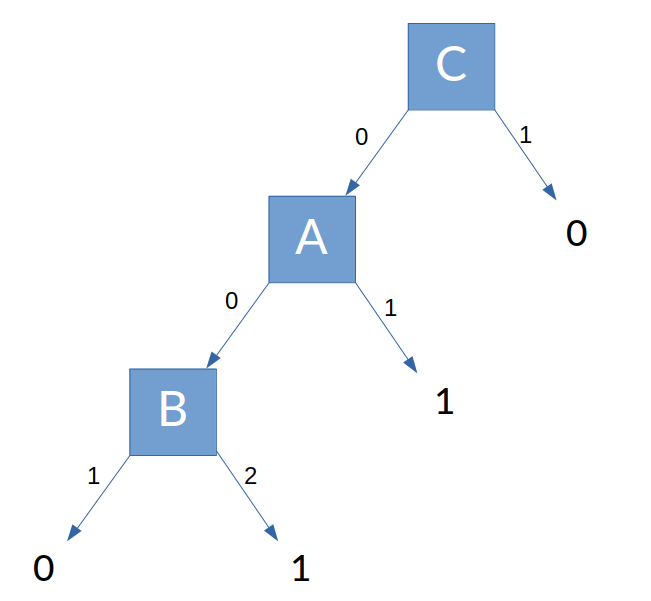
\includegraphics[width=14cm]{../code/plots/decision_tree_q8.png}
    \end{center}


    \end{your_solution}
    
\end{questions}

\clearpage

\subsection{Empirical Questions}

The following questions should be completed as you work through the programming portion of this assignment.

 \begin{questions}
    \question[3] Train and test your decision tree on the politician dataset and the education dataset with four different values of max-depth, $\{0,1,2,4\}$. Report your findings in the HW2 solutions template provided. A Decision Tree with max-depth 0 is simply a \emph{majority vote classifier}; a Decision Tree with max-depth 1 is called a \emph{decision stump}. If desired, you could even check that your answers for these two simple cases are correct using your favorite spreadsheet application (e.g. Excel, Google Sheets). (Please round each number to the fourth decimal place, e.g. 0.1234)
    
    \begin{center}
    \begin{tabular}{cc|c|c}
        % YOUR ANSWER
        \toprule
        {\bf Dataset}   & {\bf Max-Depth} & {\bf Train Error} & {\bf Test Error} \\
        \midrule
        politician & 0 & 0.443  & 0.506  \\
        politician & 1 & 0.2013  & 0.2169  \\
        politician & 2 & 0.1342  & 0.1566  \\
        politician & 4 & 0.1074  & 0.2048  \\
        \midrule
        education & 0 & 0.325  & 0.31  \\
        education & 1 & 0.195  & 0.23  \\
        education & 2 & 0.195  & 0.23  \\
        education & 4 & 0.13  & 0.155  \\
        \bottomrule
    \end{tabular}
    \end{center}
    
    
    \clearpage
    
    \question[3] For the politicians dataset, create a computer-generated plot showing error on the y-axis against depth of the tree on the x-axis. Plot \emph{both} training error and testing error, clearly labeling which is which.  That is, for each possible value of max-depth ($0, 1, 2, \ldots,$ up to the number of attributes in the dataset), you should train a decision tree and report train/test error of the model's predictions. You should include an image file below using the provided, commented out code in LaTeX, switching out \textit{politician.png} to your file name as needed.
    
        \begin{your_solution}[title=Plot,height=15cm,width=15cm]
        % YOUR ANSWER 
        \begin{center}
        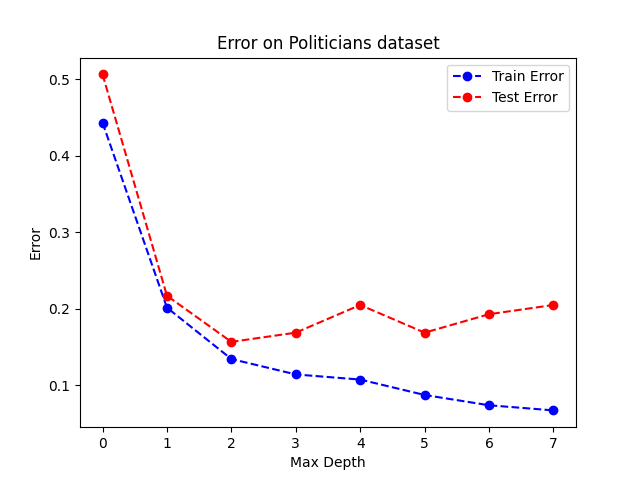
\includegraphics[width=14cm]{../code/plots/ErrorOnPoliticians.png}
        \end{center}
    \end{your_solution}


    \clearpage
    \question[3] Suppose your research advisor asks you to run some model selection experiments and then report your results. You select the Decision Tree model's max-depth to be the one with lowest test error in metrics.txt and then report that model's test error as the performance of our classifier on held out test data. Is this a good experimental setup? If so, why? If not, why not?
    

    

    
    
    \begin{your_solution}[title=Answer,height=7cm,width=15cm]
        % YOUR ANSWER 
No, I dont believe this is a good experimental setup. \newline
As the decision tree keeps training and splitting its nodes further, there comes a point after which it's no longer learning anything useful but rather is overfitting to the training data. Thus, the overall training error would continute reducing however, the tree wouldn't be generalizing well. Since the training error keeps improving regardless of whether the tree was generalizing, it would a bad choice. 
While we can observe the measured test error and choose the max\_depth value corresponding to the point where the test error and train errors are both low before diverging, it's still a bad choice as doing so would actually induce a bias. Ideally, the model should never be aware of the test data unless the final testing.\newline
The ideal choice here would be to split up the train data into train and validation data. We could use this validation data to obtain the best max\_depth by observing the errors. We could also try k-fold cross validation so that we choose the best possible max\_depth across the entire training data.    
    \end{your_solution}


\question[3] In this assignment, we used max-depth as our stopping criterion, and as a mechanism to prevent overfitting. Alternatively, we could stop splitting a node whenever the mutual information for the best attribute is lower than a threshold value. This threshold would be another hyperparameter. Theoretically, how would increasing this threshold value affect the number of nodes and depth of the learned trees?
    
    \begin{your_solution}[title=Answer,height=5cm,width=15cm]
        % YOUR ANSWER 
        The threshold parameter would prevent node splitting if the mutual information for the best attribute was lower than the threshold value. Increasing this value would, thus, increase the limit/restriction on the allowed mutual information. Thus, increasing the threshold value would restrict node splitting, leading to lesser number of nodes and a shallower tree.
However, there could be some corner cases wherein the data splits quickly and cleanly (eg. mushroom dataset). In such cases, the threshold value changes might not make a difference as the tree is not that deep to begin with. But with noisy dataset, this threshold would be a great way for early stopping.
    \end{your_solution}


    \clearpage
    \question[3] Continuing from the previous question, how would you set-up model training to choose the threshold value?
    

    \begin{your_solution}[title=Answer,height=5cm,width=15cm]
        % YOUR ANSWER 
        One way to obtain the right threshold value would be to try different ones on training and val data (split from train data). Starting from 0 (i.e. no threshold), we could perform a few experiments wherein we increase the threshold by small increments (say 0.05). For low or 0 thresholds, the train error would be low but val error would be high (overfitting). We keep increasing threshold till the val and train errors stop diverging and are both within acceptable low error margins.
Increasing the threshold further could have adverse effects - it could unnecessarily prevent node splitting thereby, not allowing tree to represent the data pattern properly.
Thus, the range of thresholds for which the val and train errors are not diverging and are both low and within acceptable error margins, would be the right choice.
    \end{your_solution}
    
    % \clearpage
    \question[2] Print (do not handwrite!) the decision tree which is produced by your algorithm for the politician data with max depth 3. Instructions on how to print the tree could be found in section \ref{sec:printtree}.
    
    \newsavebox{\outputbox}
    \setbox\outputbox=\hbox{\begin{lstlisting}	  [backgroundcolor=\transparent{0}\color{white}]
  [83 democrat/66 republican]
  | Superfund_right_to_sue = n: [55 democrat/2 republican]
  | | Export_south_africa = n: [0 democrat/1 republican]
  | | Export_south_africa = y: [55 democrat/1 republican]
  | | | Immigration = n: [46 democrat/0 republican]
  | | | Immigration = y: [9 democrat/1 republican]
  | Superfund_right_to_sue = y: [28 democrat/64 republican]
  | | Aid_to_nicaraguan_contras = n: [13 democrat/58 republican]
  | | | Export_south_africa = n: [0 democrat/20 republican]
  | | | Export_south_africa = y: [13 democrat/38 republican]
  | | Aid_to_nicaraguan_contras = y: [15 democrat/6 republican]
  | | | Mx_missile = n: [12 democrat/0 republican]
  | | | Mx_missile = y: [3 democrat/6 republican]

    \end{lstlisting}}
    
    \begin{your_solution}[title=Output,height=12cm,width=16cm]
    \hspace{-1.5cm}
    \usebox\outputbox
    

    
    \end{your_solution}
    

    \clearpage
    \question[2] Describe the decision tree for the mushrooms dataset.
    How would you differentiate between poisonous and edible mushrooms?
    

    \begin{your_solution}[title=Answer,height=5cm,width=15cm]
%The decision tree has a depth of 2 and a train error of 0.06. While allowing the decision tree to grow to a depth of 5 ensures pure leaf nodes i.e. 0 train error, the overall test error (0.0207) is higher than that at a max-depth of 2 (0.0169).
%\newline 
%Mushrooms with a foul odor are definitely poisonous. Those without a foul odor are further divided based on whether their gill size is broad.
%Those with broad gills are edible with a 97.92\% certainty while those without broad gills are poisonous with a 68.14\% certainty.
The decision tree has a depth of 5. All the leaf nodes are pure i.e. 0 entropy.\newline
	If the odor's foul, then the mushroom is poisonous while those without a foul odor are further divided based on whether their gill size is broad.
Those with broad gills and spore print color green are poisonous while those with other colors are edible.
Those without broad gills are further divided on the absence of odor. Those with odor and with close gill spacing are poisonous. Those with odor but without close gill spacing depend upon bruises - with bruises are edible and those without are poisonous. Those without odor and with silky stalk surface are poisonous. Those without odor but without a silky stalk surface further depend on bruises - those with bruises are poisonous while those without are edible.
    \end{your_solution}
    
\end{questions}

\newpage

\section{Collaboration Questions}
After you have completed all other components of this assignment, report your answers to these questions regarding the collaboration policy. Details of the policy can be found \href{http://www.cs.cmu.edu/~mgormley/courses/10601/about.html}{here}.
\begin{enumerate}
    \item Did you receive any help whatsoever from anyone in solving this assignment? Is so, include full details.
    \item Did you give any help whatsoever to anyone in solving this assignment? Is so, include full details.
    \item Did you find or come across code that implements any part of this assignment ? If so, include full details.
\end{enumerate}

\begin{your_solution}[height=6cm]
% YOUR ANSWER 
1 - No\newline
2 - No\newline
3 - No
\end{your_solution}\newpage

\section{Programming: (70 points)}

Your goal in this assignment is to implement a binary classifier, entirely from scratch--specifically a Decision Tree learner. In addition, we will ask you to run some end-to-end experiments on three tasks (predicting the party of a politician / predicting final grade for high school students / predicting whether a mushroom is poisonous) and report your results.
%
You will write two programs: \texttt{inspection.\{py|java|cpp\}} (Section \ref{sec:inspect}) and \texttt{decisionTree.\{py|java|cpp\}} (Section \ref{sec:decisiontree}). The programs you write will be automatically graded using the Gradescope system. You may write your programs in \textbf{Python}, \textbf{Java}, or \textbf{C++}. However, you should use the same language for all parts below. In general, \textbf{Python} is recommended.

\subsection{The Tasks and Datasets}
\label{sec:data}

\paragraph{Materials} Download the zip file from the course website. The zip file will have a handout folder that contains all the data that you will need in order to complete this assignment.

\paragraph{Datasets}

The handout contains four datasets. Each one contains attributes and labels and is already split into training and testing data. The first line of each \lstinline{.tsv} file contains the name of each attribute, and \emph{the class is always the last column}.

\begin{enumerate}
\item \textbf{politician:}
    The first task is to predict whether a US politician is a member of the Democrat or Republican party, based on their past voting history. Attributes (aka. features) are short descriptions of bills that were voted on, such as \emph{Aid\_to\_nicaraguan\_contras} or \emph{Duty\_free\_exports}. Values are given as \emph{`y'} for yes votes and \emph{`n'} for no votes. The training data is in \lstinline{politicians_train.tsv}, and the test data in \lstinline{politicians_test.tsv}.
\item \textbf{education:}
    The second task is to predict the final \emph{grade} (A, not A) for high school students. The attributes (covariates, predictors) are student grades on 5 multiple choice assignments \emph{M1} through \emph{M5}, 4 programming assignments \emph{P1} through \emph{P4}, and the final exam \emph{F}. The training data is in \newline \lstinline{education_train.tsv}, and the test data in \lstinline{education_test.tsv}.
\item \textbf{small:}
    We also include \lstinline{small_train.tsv} and \lstinline{small_test.tsv}---a small, purely for demonstration version of the politicians dataset, with \emph{only} attributes \emph{Anti\_satellite\_test\_ban} and \newline \emph{Export\_south\_africa}.  
    For this small dataset, the handout tar file also contains the predictions from a reference implementation of a Decision Tree with max-depth 3 (see \lstinline{small_3_train.labels}, \lstinline{small_3_test.labels}, \lstinline{small_3_metrics.txt}).
    You can check your own output against these to see if your implementation is correct.\footnote{Yes, you read that correctly: we are giving you the correct answers.}
\item \textbf{mushrooms:}
    Finally, we have a large dataset of mushroom samples, \lstinline{mushrooms_train.tsv} and \lstinline{mushrooms_test.tsv},
    for you to test your algorithm against.
    Each sample has discrete attributes which were split into boolean attributes. For example, \emph{cap-size} could be  \emph{bell}, \emph{conical}, \emph{convex}, \emph{flat}, \emph{knobbed}, or \emph{sunken}. This was split into boolean attributes \emph{cap-size\_bell}, \emph{cap-size\_conical},  \emph{cap-size\_convex}, etc.
    Your goal is to differentiate the poisonous versus edible mushrooms.
\end{enumerate}

\begin{notebox} \textbf{Note:}
For simplicity, all attributes are discretized into just two categories (i.e. each node will have at most two descendents). This applies to all the datasets in the handout, as well as the additional datasets on which we will evaluate your Decision Tree.
\end{notebox}

\newpage
\subsection{Program \#1: Inspecting the Data [5pts]}
\label{sec:inspect}

    Write a program \texttt{inspection.\{py|java|cpp\}} to calculate the label entropy at the root (i.e. the entropy of the labels before any splits) and the error rate (the percent of incorrectly classified instances) of classifying using a majority vote (picking the label with the most examples). You do not need to look at the values of any of the attributes to do these calculations, knowing the labels of each example is sufficient. \textbf{Entropy should be calculated in bits using log base 2.}

\paragraph{Command Line Arguments}
The autograder runs and evaluates the output from the files  generated, using the following command:

\begin{tabular}{ll}
 For Python:
 &
\begin{lstlisting}[language=Shell]
$ python3 inspection.py <input> <output>
\end{lstlisting}
\\
For Java:
&
\begin{lstlisting}[language=Shell]
$ javac inspection.java; java inspect <input> <output>
\end{lstlisting}
\\

% For C:
% \begin{lstlisting}[language=Shell]
% $ gcc inspect.c; ./a.out <input> <output>
% \end{lstlisting}
For C++:
&
\begin{lstlisting}[language=Shell]
$ g++ inspection.cpp; ./a.out <input> <output>
\end{lstlisting}
\\
\end{tabular}

Your program should accept two command line arguments: an input file and an output file. It should read the \lstinline{.tsv} input file (of the format described in Section \ref{sec:data}), compute the quantities above, and write them to the output file so that it contains:
\begin{quote}
\begin{verbatim}
entropy: <entropy value>
error: <error value>
\end{verbatim}
\end{quote}

\paragraph{Example}

For example, suppose you wanted to inspect the file \lstinline{small_train.tsv} and write out the results to \lstinline{small_inspect.txt}. For Python, you would run the command below:
%
\begin{lstlisting}[language=Shell]
$ python3 inspection.py small_train.tsv small_inspect.txt
\end{lstlisting}
%
Afterwards, your output file \lstinline{small_inspect.txt} should contain the following:
%
\begin{quote}
\begin{verbatim}
entropy: 0.996316519559
error: 0.464285714286
\end{verbatim}
\end{quote}
%
Our autograder will run your program on several input datasets to check that it correctly computes entropy and error, and will take minor differences due to rounding into account. You do not need to round your reported numbers! The Autograder will automatically incorporate the right tolerance for float comparisons.

\begin{notebox}
For your own records, run your program on each of the datasets provided in the handout---this error rate for a \emph{majority vote} classifier is a baseline over which we would (ideally) like to improve.
\end{notebox}

\newpage
\subsection{Program \#2: Decision Tree Learner [65pts]}
\label{sec:decisiontree}

In decisionTree.\{py $\mid$ java $\mid$ cpp\}, implement a Decision Tree learner. This file should learn a decision tree with a specified maximum depth, print the decision tree in a specified format, predict the labels of the training and testing examples, and calculate training and testing errors.

\textbf{Your implementation must satisfy the following requirements:}
\begin{itemize}
\item Use mutual information to determine which attribute to split on.
\item Be sure you’re correctly weighting your calculation of mutual information. For a split on attribute X, $I(Y;X) = H(Y)-H(Y|X) = H(Y) - P(X=0)H(Y|X = 0) - P(X = 1)H(Y|X = 1)$.
\item As a stopping rule, only split on an attribute if the mutual information is $>$ 0. 
\item You should split with replacement. That is, when you split on a column, you should retain this column in child datasets. 
\item Do not grow the tree beyond a max-depth specified on the command line. For example, for a maximum depth of 3, split a node only if the mutual information is $>$ 0 and the current level of the node is $< 3$.
\item Use a majority vote of the labels at each leaf to make classification decisions. If the vote is tied, choose the label that comes \textbf{\textit{last}} in the lexicographical order (i.e. Republican should be chosen before Democrat)
\item It is possible for attributes to have equal values for mutual information. In this case, you should split on the first attribute to break ties.
\item Do not hard-code any aspects of the datasets into your code. We may autograde your programs on hidden datasets that include different attributes and output labels.
\end{itemize}

Careful planning will help you to correctly and concisely implement your Decision Tree learner. Here are a few \emph{hints} to get you started:
\begin{itemize}
    \item Write helper functions to calculate entropy and mutual information.
    \item Write a function to train a stump (tree with only one level). Then call that function recursively to create the sub-trees.
    \item In the recursion, keep track of the depth of the current tree so you can stop growing the tree beyond the max-depth.
    \item Implement a function that takes a learned decision tree and data as inputs, and generates predicted labels. You can write a separate function to calculate the error of the predicted labels with respect to the given (ground-truth) labels.
    \item Be sure to correctly handle the case where the specified maximum depth is greater than the total number of attributes.
    \item Be sure to handle the case where max-depth is zero (i.e. a majority vote classifier). 
    \item Look under the FAQ's on Piazza for more useful clarifications about the assignment.
\end{itemize}

\subsection{Command Line Arguments}

The autograder runs and evaluates the output from the files  generated, using the following command:

\begin{tabular}{ll}
For Python: &
\begin{lstlisting}[language=Shell]
$ python3 decisionTree.py [args...]
\end{lstlisting}
\\
For Java: &
\begin{lstlisting}[language=Shell]
$ javac decisionTree.java; java decisionTree [args...]
\end{lstlisting}
\\
For C++: &
\begin{lstlisting}[language=Shell]
$ g++ -g decisionTree.cpp -o decisionTree; ./decisionTree [args...]
\end{lstlisting}
\end{tabular}

Where above \lstinline{[args...]} is a placeholder for six command-line arguments: 
\texttt{<train input> <test input> <max depth> <train out> <test out> <metrics out>}. These arguments are described in detail below:
\begin{enumerate}
\item \lstinline{<train input>}: path to the training input \lstinline{.tsv} file (see Section \ref{sec:data})
\item \lstinline{<test input>}: path to the test input \lstinline{.tsv} file (see Section \ref{sec:data})
\item \lstinline{<max depth>}: maximum depth to which the tree should be built
\item \lstinline{<train out>}: path of output \lstinline{.labels} file to which the predictions on the \textit{training} data should be written (see Section \ref{sec:labels})
\item \lstinline{<test out>}: path of output \lstinline{.labels} file to which the predictions on the \emph{test} data should be written (see Section \ref{sec:labels})
\item \lstinline{<metrics out>}: path of the output \lstinline{.txt} file to which metrics such as train and test error should be written (see Section \ref{sec:metrics})
\end{enumerate}

As an example, if you implemented your program in Python, the following command line would run your program on the politicians dataset and learn a tree with max-depth of two. The train predictions would be written to \lstinline{pol_2_train.labels}, the test predictions to \lstinline{pol_2_test.labels}, and the metrics to \lstinline{pol_2_metrics.txt}.
%
\begin{lstlisting}[language=Shell]
$ python3 decisionTree.py politicians_train.tsv politicians_test.tsv \ 
        2 pol_2_train.labels pol_2_test.labels pol_2_metrics.txt
\end{lstlisting}
%
The following example would run the same learning setup except with max-depth three, and conveniently writing to analogously named output files, so you can can compare the two runs.
%
\begin{lstlisting}[language=Shell]
$ python3 decisionTree.py politicians_train.tsv politicians_test.tsv \ 
        3 pol_3_train.labels pol_3_test.labels pol_3_metrics.txt
\end{lstlisting}

\subsection{Output: Labels Files}
\label{sec:labels}

Your program should write two output \lstinline{.labels} files containing the predictions of your model on training data (\lstinline{<train out>}) and test data (\lstinline{<test out>}). Each should contain the predicted labels for each example printed on a new line. Use `\textbackslash n' to create a new line.

Your labels should exactly match those of a reference decision tree implementation---this will be checked by the autograder by running your program and evaluating your output file against the reference solution.

\textbf{Note}: You should output your predicted labels using the same string identifiers as the original training data: e.g., for the politicians dataset you should output democrat/republican and for the education dataset you should output A/notA.
%
The first few lines of an example output file is given below for the politician dataset:
\begin{quote}
\begin{verbatim}
democrat
democrat
democrat
republican
democrat
...
\end{verbatim}
\end{quote}

\subsection{Output: Metrics File}
\label{sec:metrics}

Generate another file where you should report the training error and testing error. This file should be written to the path specified by the command line argument \lstinline{<metrics out>}. Your reported numbers should be within 0.01 of the reference solution. You do not need to round your reported numbers! The Autograder will automatically incorporate the right tolerance for float comparisons. The file should be formatted as follows:

\begin{quote}
\begin{verbatim}
error(train): 0.0714
error(test): 0.1429
\end{verbatim}
\end{quote}

The values above correspond to the results from training a tree of depth 3 on \texttt{small\_train.tsv} and testing on \texttt{small\_test.tsv}. (There is one space between the colon and value)


\subsection{Output: Printing the Tree}
\label{sec:printtree}

Finally, you should write a function to pretty-print your learned decision tree. (You may find it more convenient to print the tree \emph{as} you are learning it.) Each row should correspond to a node in the tree. They should be printed in a \emph{depth-first-search} order (but you may print left-to-right or right-to-left, i.e. your answer do not need to have exactly the same order as the reference below). Print the attribute of the node's parent and the attribute value corresponding to the node. Also include the sufficient statistics (i.e. count of positive / negative examples) for the data passed to that node. The row for the root should include \emph{only} those sufficient statistics. A node at depth $d$, should be prefixed by $d$ copies of the string `$\mid$ '.

Below, we have provided the recommended format for printing the tree (example for python). You can print it directly to standard out rather than to a file. \textbf{This functionality of your program will not be autograded}.

\begin{lstlisting}[language=Shell]
$ python3 decisionTree.py small_train.tsv small_test.tsv 2 \ 
small_2_train.labels small_2_test.labels small_2_metrics.txt

[15 democrat/13 republican]
| Anti_satellite_test_ban = y: [13 democrat/1 republican]
| | Export_south_africa = y: [13 democrat/0 republican]
| | Export_south_africa = n: [0 democrat/1 republican]
| Anti_satellite_test_ban = n: [2 democrat/12 republican]
| | Export_south_africa = y: [2 democrat/7 republican]
| | Export_south_africa = n: [0 democrat/5 republican]
\end{lstlisting}

However, you should be careful that the tree might not be full. For example, after swapping the train/test files in the example above, you could end up with a tree like the following.

\begin{lstlisting}[language=Shell]
$ python3 decisionTree.py small_test.tsv small_train.tsv 2 \ 
swap_2_train.labels swap_2_test.labels swap_2_metrics.txt

[13 democrat/15 republican]
| Anti_satellite_test_ban = y: [9 democrat/0 republican]
| Anti_satellite_test_ban = n: [4 democrat/15 republican]
| | Export_south_africa = y: [4 democrat/10 republican]
| | Export_south_africa = n: [0 democrat/5 republican]
\end{lstlisting}

The following pretty-print shows the education dataset with max-depth 3.  Use this example to check your code before submitting your pretty-print of the politics dataset (asked in question 14 of the Empirical questions).  

\begin{lstlisting}[language=Shell]
$ python3 decisionTree.py education_train.tsv education_test.tsv 3 \
edu_3_train.labels edu_3_test.labels edu_3_metrics.txt

[135 A/65 notA]
| F = A: [119 A/23 notA]
| | M4 = A: [56 A/2 notA]
| | | P1 = A: [41 A/0 notA]
| | | P1 = notA: [15 A/2 notA]
| | M4 = notA: [63 A/21 notA]
| | | M2 = A: [37 A/3 notA]
| | | M2 = notA: [26 A/18 notA]
| F = notA: [16 A/42 notA]
| | M2 = A: [13 A/15 notA]
| | | M4 = A: [6 A/1 notA]
| | | M4 = notA: [7 A/14 notA]
| | M2 = notA: [3 A/27 notA]
| | | M4 = A: [3 A/5 notA]
| | | M4 = notA: [0 A/22 notA]
\end{lstlisting}

The numbers in brackets give the number of positive and negative labels from the training data in that part of the tree.

\begin{notebox}
At this point, you should be able to go back and answer questions 1-7 in the "Empirical Questions" section of this handout.  Write your solutions in the template provided. 
\end{notebox}

\begin{comment}
    \subsection{Evaluation}
    In addition to the politician and education datasets, our autograder will test your code on two more datasets, which will not be shown to you. One set contains information about various cars, and whether or not consumers decided to buy them. The other contains data about songs, and whether or not they became top hits. The data will be in .tsv files formatted like the ones provided, again with the class as the last column. Shown below are the attributes and the values they can take: 
    
    Music data:
    
    \begin{itemize}
    \item \texttt{Attribute:year('before1950'or'after1950')}
    \item \texttt{Attribute:solo('yes'or'no')}
    \item \texttt{Attribute:vocal('yes'or'no')}
    \item \texttt{Attribute:length('morethan3min'or'lessthan3min')}
    \item \texttt{Attribute:original('yes'or'no')}
    \item \texttt{Attribute:tempo('fast'or'slow')}
    \item \texttt{Attribute:folk('yes'or'no')}
    \item \texttt{Attribute:classical('yes'or'no')}
    \item \texttt{Attribute:rhythm('yes'or'no')}
    \item \texttt{Attribute:jazz('yes'or'no')}
    \item \texttt{Attribute:rock('yes'or'no')}
    \item \texttt{Class Label:hit('yes'or'no')}
    \end{itemize}
    
    Cars data:
    
    \begin{itemize}
    \item \texttt{Attribute:buying('expensive'or'cheap')}
    \item \texttt{Attribute:maint('high'or'low')}
    \item \texttt{Attribute:doors('Two'or'MoreThanTwo')}
    \item \texttt{Attribute:length('morethan3min'or'lessthan3min')}
    \item \texttt{Attribute:person('Two'or'MoreThanTwo')}
    \item \texttt{Attribute:boot('large'or'small')}
    \item \texttt{Attribute:safety('high'or'low')}
    \item \texttt{Class Label:class('yes'or'no')}
    \end{itemize}
    
    Please ensure your solution can handle data with these values.
 
\end{comment}
    
\subsection{Submission Instructions}

\paragraph{Programming}
Please ensure you have completed the following files for submission.


\begin{verbatim}
inspection.{py|java|cpp}
decisionTree.{py|java|cpp}
\end{verbatim}

When submitting your solution, make sure to select and upload both files. Ensure the files have the exact same spelling and letter casing as above. You can either directly zip the two files (by selecting the two files and compressing them - do not compress the folder containing the files) or directly drag them to Gradescope for submission.


\textbf{Note}: Please make sure the programming language that you use is consistent within this assignment (e.g. don't use C++ for inspect and Python for decisionTree).

\paragraph{Written Questions}
Make sure you have completed all questions from Written component (including the collaboration policy questions) in the template provided.  When you have done so, please submit your document in \textbf{pdf format} to the corresponding assignment slot on Gradescope.



\newpage

\end{document}